	\documentclass[10pt,oneside]{CBFT_book}
	% Algunos paquetes
	\usepackage{amssymb}
	\usepackage{amsmath}
	\usepackage{graphicx}
% 	\usepackage{libertine}
% 	\usepackage[bold-style=TeX]{unicode-math}
	\usepackage{lipsum}

	\usepackage{natbib}
	\setcitestyle{square}

	\usepackage{polyglossia}
	\setdefaultlanguage{spanish}
	

	\everymath{\displaystyle}

	\usepackage{CBFT.estilo} % Cargo la hoja de estilo

	% Tipografías
	% \setromanfont[Mapping=tex-text]{Linux Libertine O}
	% \setsansfont[Mapping=tex-text]{DejaVu Sans}
	% \setmonofont[Mapping=tex-text]{DejaVu Sans Mono}

	%===================================================================
	%	DOCUMENTO PROPIAMENTE DICHO
	%===================================================================

\begin{document}

% =================================================================================================
\chapter{Introducción al momento angular (rotaciones)}
% =================================================================================================

El operador $\hat{L}$ será el encargado de realizar las rotaciones. Por el álgebra visto en la mecánica 
clásica sabemos que, dado un vector \vb{v} y una matriz ortogonal $R$ se tiene
\[
	\vb{v}' = R \vb{v} \qquad \text{con} \quad |\vb{v}'|=|\vb{v}|
\]
y 
\[
	|\vb{v}|^2 = V^t V = (V^t R^t) (R V) \qquad \text{pues} \quad R^tR=RR^t = \mathbb{1}
\]
puesto que es una matriz ortogonal.
Una matriz ortogonal tiene tres parámetros independientes.
Luego se cumplen 
\begin{itemize}
 \item Clausura 
 \[
	(R_1R_2)(R_1R_2)^t = R_1R_2R_2^tR_1^t = \mathbb{1}
\]
\item El producto de dos matrices ortogonales es otra matriz ortogonal (aquella que cumple $R^rR=\mathbb{1}$).
Asociatividad
\[
	R_1(R_2R_3) = (R_1R_2)R_3
\]
\item Existencia de identidad
\[
	R \: \mathbb{1} = \mathbb{1}R = R
\]
\item Existencia de inversa
\[
	R \: R^{-1} = R^{-1}R = \mathbb{1} \qquad \text{con}\; R^{-1}\equiv R^t
\]
\end{itemize}

Esto define un grupo de matrices ortogonales que realiza rotaciones y se denomina $SO(3)$.
Las rotaciones son un grupo respecto a la multiplicación.

\subsection{No conmutatividad de las rotaciones clásicas}

Las rotaciones finitas no conmutan. Luego, el grupo de las rotaciones será un grupo abeliano
\[
	R_z(\varphi) = \begin{pmatrix}
	\cos(\varphi) & -\sin(\varphi) & 0 \\
	\sin(\varphi) & \cos(\varphi) & 0 \\
	0 & 0 & 1
	\end{pmatrix}
\]
\[
	R_x(\varphi) = \begin{pmatrix}
	1 & 0 & 0 \\
	0 & \cos(\varphi) & -\sin(\varphi) \\
	0 & \sin(\varphi) & \cos(\varphi)
	\end{pmatrix}
\]
\[
	R_y(\varphi) = \begin{pmatrix}
	\cos(\varphi) & 0 & \sin(\varphi) \\
	0 & 1 & 0 \\
	-\sin(\varphi) & 0 & \cos(\varphi)
	\end{pmatrix}
\]

\begin{figure}[!htb]
	\begin{center}
	\includegraphics[width=0.4\textwidth]{images/teo2_10.pdf}
	\end{center}
	\caption{}
\end{figure} 

Si reemplazamos $\cos(\epsilon) \approx 1 - \epsilon^2/2$ y $\sin(\epsilon) \approx \epsilon$ hasta orden dos.
Se puede ver que las rotaciones, en torno a ejes diferentes, sólo conmutan a orden uno $(\epsilon)$ de manera 
que una rotación infinitesimal $d\varphi$ conmuta pero una rotación finita $\varphi$ no lo hace.

En efecto, hasta orden 2 se tienen 
\[
	R_z(\epsilon) = \begin{pmatrix}
	1 - \epsilon^2/2 & - \epsilon  & 0 \\
	\epsilon & 1 - \epsilon^2/2 & 0 \\
	0 & 0 & 1
	\end{pmatrix}
\]
\[
	R_x(\epsilon) = \begin{pmatrix}
	1 & 0 & 0 \\
	0 & 1 - \epsilon^2/2 & -\epsilon \\
	0 & \epsilon & 1 - \epsilon^2/2
	\end{pmatrix}
\]
\[
	R_y(\epsilon) = \begin{pmatrix}
	1 - \epsilon^2/2 & 0 & \epsilon \\
	0 & 1 & 0 \\
	-\epsilon & 0 & 1 - \epsilon^2/2
	\end{pmatrix}
\]

Entonces, se ve que
\[
	R_x(\epsilon) R_y(\epsilon) - R_y(\epsilon) R_x(\epsilon) = 
	\begin{pmatrix}
	0 & -\epsilon^2  & 0 \\
	\epsilon^2 & 0 & 0 \\
	0 & 0 & 0
	\end{pmatrix}	
\]
o bien
\[
	[ R_x(\epsilon), R_y(\epsilon) ] =  R_z(\epsilon) - \mathbb{1}
\]

Como el conmutador es diferente de cero el grupo de las rotaciones es un grupo no abeliano.
La velocidad angular se define $\d\omega/dt$ de modo que eso justifica que los vectores
velocidad angular puedan sumarse en mecánica.
Esto es lo que sucedía en el caso clásico. Veamos ahora qué le pasa a los kets ante rotaciones.

% =================================================================================================
\section{Rotaciones cuánticas}
% =================================================================================================

Para las rotaciones cuánticas suponemos la existencia de un operador $D_R$ que las realiza, que
convierte $ \Ket{\a} \to \Ket{\a}_R $ con $ \Ket{\a}_R = D(R) \Ket{\a} $ postulándose una forma del
tipo 
\[
	D(\hat{n},d\phi) = \mathbb{1} - i \frac{\vb{J}\cdot\hat{n}}{\hbar}d\phi,
\]
para una rotación infinitesimal o bien
\[
	D(\hat{n},\theta) = \lim_{N\to\infty} \left( 1 - \frac{i J_z \theta}{\hbar N} \right)^N =
	\euler^{-i \vb{J}\cdot\hat{n} \theta / \hbar },
\]
para rotación finita. 

Otro modo de ver esto, es considerando 
\[
	D_R(\nver,\theta + d\theta) = D_R(\nver,\theta) D_R(\nver,d\theta) 
	= D_R(\nver,\theta) \left[ \mathbb{1} - \frac{i}{\hbar} d\theta \: \pe{J}{\nver}\right]
\]
de modo que
\[
	\frac{ D_R(\nver,\theta + d\theta) -D_R(\nver,\theta) }{d\theta} = 
	\frac{i}{\hbar} \:\pe{J}{\nver} D_R(\nver,\theta) 
\]
lo que conduce a
\[
	\dpar{}{\theta} D_R(\nver,\theta) = - \frac{i}{\hbar} \:\pe{J}{\nver} \: D_R(\nver,\theta)
\]
y, usando la condición de contorno de que $D_R(\nver,0) = \mathbb{1}$ se tiene
\[
	D_R(\nver,\theta) = \euler^{-i /\hbar \: \theta (\pe{J}{\nver}) },
\]
junto con la relación de conmutación $ [J_i, J_j] = i \hbar \epsilon_{ijk} J_k $.

$\hat{D}$ es, como se dijo, el operador de las rotaciones y $\hat{J}$ es un momento angular 
general. Se postula de esta forma para que $\hat{D}$ cumpla las mismas propiedades que $R$ y la 
misma relación de conmutación (lo cual los hace pertenecer al mismo álgebra)
\[
	R_x R_y - R_y R_x = R_z (\epsilon^2) - \mathbb{1}
\]
\[
	D(\hat{x},\epsilon) D(\hat{y},\epsilon) - D(\hat{y},\epsilon) D(\hat{x},\epsilon) =
	D(\hat{z},\epsilon^2) - D(\mathbb{1})
\]
de modo que la cuenta lleva a  
\[
	J_x J_y - J_y J_x = i \hbar J_z
\]
la cual generalizando se llega a 
\be
	[J_i,J_j] = i \hbar \epsilon_{ijk} J_k
	\label{conmutacion_J}
\ee
que son las relaciones de conmutación generales para momento angular $\hat{J}$.
Esto vale para cualquier rotación, lo cual es más amplio que si es solo $L$, el momento angular.

\begin{ejemplo}{\bf Operador de rotación para partículas de spin 1/2}
 
Para sistemas de spín $1/2$ es 
\[
	D(\hat{n},\phi) \equiv \euler^{-i/\hbar \vb{S}\cdot\hat{n} }
\] 
El efecto de la rotación se asocia a 
\[
	_R\Braket{\a|S_x|\a}_R = \Braket{ \a | \euler^{i S_z \phi /\hbar} 
	\: S_x \: \euler^{-i S_z \phi /\hbar}  | \a }
\]
una cosa que podemos considerar como un operador y los kets fijos en el tiempo.
La base de autoestados de $S_z$ es 
\[
	S_z\Ket{+} = \frac{\hbar}{2}\Ket{+} \qquad \qquad 
	S_z\Ket{-} = -\frac{\hbar}{2}\Ket{-}
\]
los operadores $S_x, S_y, S_z$ tienen sus expresiones usuales y evaluando resulta
\[
	D^\dagger \: S_x \: D =
	\frac{\hbar}{2} 
	\left[
	( \KB{+}{-} + \KB{-}{+} ) \cos\phi + i ( \KB{+}{-} - \KB{-}{+}  )\sin \phi 
	\right]
\]
que es como si el vector $S_x$ se transformase como lo haría un vector. En efecto,
se tiene
\[
	S_x \qquad \to \text{rotación} \to \qquad S_x \cos\phi - S_y \sin\phi
\]
\[
	S_y \qquad \to \text{rotación} \to \qquad S_y \cos\phi + S_x \sin\phi
\]
pero 
\[
	S_z \qquad \to \text{rotación} \to \qquad S_z
\]
lo cual se demuestra por conmutación en la expresión del operador.
 
Se puede ver que ante rotaciones cuánticas $D(\hat{n},\phi)$ los valores de expectación transforman como 
vectores
\[
	\begin{pmatrix} \Braket{S_x'} \\ \Braket{S_y'} \\ \Braket{S_z'}	\end{pmatrix} =	\begin{pmatrix} 
	\\
	 R(\hat{x},\phi) \\
	 \\
	\end{pmatrix}\begin{pmatrix} \Braket{S_x} \\ \Braket{S_y} \\ \Braket{S_z} \end{pmatrix}
\]

En general $\vb{J} = (J_x, J_y, J_z)$ se transforma como vector y entonces $\hat{J}$ es un operador vectorial.
Consideremos un estado de un sistema de spín $1/2$,
\[
	\Ket{\alpha} = \Braket{+|\alpha}\Ket{+} + \Braket{-|\alpha}\Ket{-}
\]
\[
	D(\hat{z},\phi)\Ket{\alpha} = \euler^{-iS_z\phi/\hbar}\Braket{+|\alpha}\Ket{+} +
		\euler^{-iS_z\phi/\hbar} \Braket{-|\alpha}\Ket{-}
\]
\[
	D(\hat{z},\phi)\Ket{\alpha} = \Braket{+|\alpha} \euler^{-i\phi/2} \Ket{+} +
		\euler^{i\phi/2} \Braket{-|\alpha}\Ket{-}
\]
Haciendo una rotación de $\phi=2\pi$ (cosa que debiera dejar al ket incólume) se tiene 
\[
	D(\hat{z},2\pi) \Ket{\alpha} = - \Braket{+|\alpha}\Ket{+} - \Braket{-|\alpha}\Ket{-} = -\Ket{\alpha}
\]

Luego, esto es una muestra del carácter no-clásico del spin; una vuelta completa le cambia el signo al ket 
pero notemos cuidadosamente que el valor de expectación -- que es algo físico -- no varía. Esto muestra que 
el ket no puede tener sentido físico.

Se observó en 1975 que el patrón de interferencia se altera con el $-\Ket{\a}$ de manera que tiene 
importancia ese signo en el ket.

En la picture se esquematiza. Hay necutrones a la izquierda y un campo magnético $\vb B$ delante de la
parted. Se ve en la interferencia que llega con el signo cambiado; le hacen dar una vuelta completa
al spin.

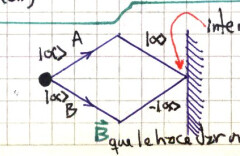
\includegraphics[width=0.20\textwidth]{images/fig_ft2_spin12_rotaciones_experimento.jpg}

\end{ejemplo}

\subsection{Angulos de Euler}

Se define una serie de rotaciones 
\[
	1.\; R_{z}(\alpha) \qquad 2.\; R_{y'}(\beta)\qquad 3.\; R_{z'}(\gamma)
\]
lo cual equivale a
\[
	R(\alpha,\beta,\gamma) = R_{z'}(\gamma) R_{y'}(\beta) R_{z}(\alpha)
\]
\notamargen{Recordemos que en general no se sabe cómo acctúan los operadores sobre un
estado general sino sobre autoestados.}
\[
	\euler^{-i J_{z'}\gamma/\hbar} \euler^{-i J_{y'}\beta/\hbar}  \euler^{-i J_z\alpha/\hbar} 
	\Ket{\psi}
\]
\begin{figure}[!htb]
	\begin{center}
	\includegraphics[width=0.4\textwidth]{images/teo2_11.pdf}
	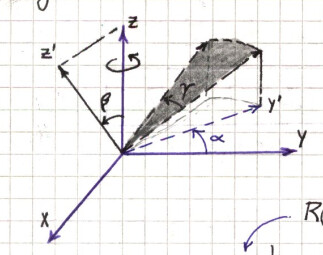
\includegraphics[width=0.4\textwidth]{images/fig_ft2_convencion_euler_angles.jpg}
	\end{center}
	\caption{Los ángulos de Euler son una caracterización de una rotación general en 3D.}
\end{figure} 
Pero desconozco cómo operar en los ejes móviles $z',y'$ así que buscaré escribir las rotaciones 
de manera que se pueda hacer la cuenta, refiriéndolas a ejes fijos.
\[
	R_{y'}(\beta) = R_{z}(\alpha) R_{y}(\beta) R_{z}^{-1}(\alpha) 
\]
\[
	R_{z'}(\gamma) = R_{y'}(\beta) R_{z}(\gamma) R_{y'}^{-1}(\beta) 
\]
siendo estas dos expresiones generales (puede probarse)
\[
	R(\alpha,\beta,\gamma) =
	R_{y'}(\beta) R_{z}(\gamma) \underbrace{R_{y'}^{-1}(\beta)R_{y'}(\beta)}_{\mathbb{1}}R_{z}(\alpha) 
\]
\[
	R(\alpha,\beta,\gamma) =
	R_{z}(\alpha) R_{y}(\beta) R_{z}^{-1}(\alpha) R_{z}(\gamma) R_{z}(\alpha)  
\]
donde las que son sobre el mismo eje conmutan y entonces,
\[
	R(\alpha,\beta,\gamma) = R_{z}(\alpha) R_{y}(\beta) R_{z}(\gamma).
\]
Rotación equivalente a [1] pero para ejes fijos, puesto que en mecánica cuántica sabemos rotar en torno a 
ejes fijos.

Los ángulos de Euler son la caracterización de una rotación general en 3D.
Entonces nuestra rotación en 3D cuántica será:
\[
	D(\alpha,\beta,\gamma) = D_z(\alpha) D_y(\beta) D_z(\gamma)  =
	\euler^{-i J_z\alpha/\hbar} \euler^{-i J_y\beta/\hbar} \euler^{-i J_z\gamma/\hbar}
\]

La ley de clausura no era tan obvia (el hecho de pedirla) [cuál es?].
No es una trivialidad como sí podrían serlo las otras tres propiedades.

El hecho de que si $R_1 R_2 = R_3$ se pasaba a los operadores $D$, de acuerdo con $ D(R_1) D(R_2) = D(R_3)$ 
solamente si los operadores $J$ verificaban la relación de conmutación dada por la Ec. \eqref{conmutacion_J}.
La información contenida en dicha relación proporciona todo lo necesario acerca del sistema.

\begin{ejemplo}{\bf Ejercicio 7}
 
Consideramos 
\[
	\Ket{a}_R = \euler^{ - i /\hbar \: S_z \vp } \Ket{\a}
\]
y se pide el valor medio $\vm{S_x}_R$ que será
\[
	_R\Braket{\a|S_x|\a}_R = \Bra{\a} \euler^{i /\hbar \: S_z \vp } \:
		S_x \: \euler^{-i /\hbar \: S_z \vp } \Ket{\a}
\]
y podemos usar la expresión de $S_x$ de la guía primera con lo cual, operando,
resulta
\[
	\vm{S_x}_R = \frac{\hbar}{2}
	\Bra{\a}
	\left( \cos\vp (\KB{+}{-} + \KB{-}{+}) + i \sin\vp (\KB{+}{-} - \KB{-}{+}) \right)
	\Ket{\a}
\]
o bien
\[
	\vm{S_x}_R = \vm{S_x} \cos\vp - \vm{S_y} \sin\vp
\]
y vemos que el valor medio del estado rotado es proyección de los valores medios
de los estados no rotados.

La parte b) fija el ángulo de la rotación en $\vp=2\pi$, luego
\[
	\Ket{\a}_R = \euler^{-i/\hbar \: 2\pi S_z} \Ket{\a}
\]
y, incorporando una constante de normalización $c$, se tiene
\[
	\euler^{-i/\hbar \: 2\pi S_z} c ( a \Ket{+} + b \Ket{-} ) =
	c ( \euler^{-i\pi} a \Ket{+} + \euler^{i\pi} b \Ket{-} ) = - \Ket{\a}
\]
y entonces vemos que rotar en $2\pi$ ha hecho aparece un signo menos.
 
\end{ejemplo}

\begin{ejemplo}{\bf Ejercicio 8}

La parte a) está hecha en el libro de Sakurai.
La parte b) pide
\[
	\euler^{-i/\hbar \: \pe{S}{\nver} \: \phi } =
	\sum_{n=0}^\infty \: \frac{(-i)^n}{n!} \phi^2 \Frac{1}{2}^n (\vb{\sigma}\cdot\nver)^n
\]
donde 
\[
	\pe{S}{\nver} = \frac{\hbar}{2} \vb{\sigma}\cdot\nver
\]
y uso representación $+ -$. Se tiene
\[
	\sum_{n=0}^\infty \: \frac{(-i)^n}{n!} \Frac{\phi}{2}^n (\vb{\sigma}\cdot\nver)^n
\]
que con $n=0$ da $\vb{\sigma}\cdot\nver=1$ y con $n=1 $ ya tenemos el producto escalar entre
$\vb{\sigma}$ y $\nver$. Con $n=2$ es
\[
	( \sigma\cdot a )( \sigma\cdot b ) = ab + i \sigma(a\times b)
\]
y con $n=3$ es similar a $n=1$ mientras que $n=4$ es similar a $n=2$. Vemos que
\[
	\vb{\sigma}\cdot\nver = \begin{cases}
		1		& \text{ par } \\
		\boldmath{\sigma}\cdot n & \text{ impar}
	\end{cases}
\]

Entonces, la sumatoria puede dividirse en dos
\[
	\sum_{n=0}^\infty \: \frac{(-i)^{2n}}{(2n)!} \Frac{\phi}{2}^{2n} +
	\sum_{n=0}^\infty \: \frac{(-i)^{2n+1}}{(2n+1)!} \Frac{\phi}{2}^n (\vb{\sigma}\cdot\nver)
\]
que da
\be
	\mathbb{1} \cos\Frac{\phi}{2} - i \: \sin\Frac{\phi}{2} ( \vb{\sigma}\cdot\nver ).
	\label{expr_rotacion}
\ee

Finalmente, el operador de rotación en la representación $\Ket{+}, \Ket{-}$ es
\[
	D(\nver,\phi) = 
	\begin{pmatrix}
	\cos\Frac{\phi}{2} - i \sin\Frac{\phi}{2} n_z	&  -( n_y + i n_x) \sin\Frac{\phi}{2} \\
			\\
	( n_y - i n_x) \sin\Frac{\phi}{2} &  \cos\Frac{\phi}{2} + i \sin\Frac{\phi}{2} n_z \\
	\end{pmatrix}
\]

La parte d) involucra primeramente una rotación alrededor de $\yver$ en $\beta$ (lo saco
de $\zver$) y en segundo lugar una rotación alrededor de $\zver$ en $\a$.
Recordemos que las rotaciones no conmutan.

Entonces, usando las expresiones anteriores de la rotación \eqref{expr_rotacion} resulta
\[
	D_R(z,\a) D_R(y,\b) \Ket{+} = 
	\cos\Frac{\b}{2} \Ket{+} + \euler^{i\a} : \sin\Frac{\b}{2}  \Ket{-}.
\]

\notamargen{Si roto primero en $\zver$ no lo saco en $z$ y no sirve a los efectos.
Esto por la no conmutatividad.}
 
\end{ejemplo}

\begin{ejemplo}{\bf Ejercicio 2}

La parte a) son cuentas fáciles (de las que le hubieran gustado a Piuselli).

La parte b) implica
\[
	U = \frac{ a_0 + i \vb{\sigma}\cdot\vb{a} }{ a_0 - i \vb{\sigma}\cdot\vb{a} }
	= \frac{ (a_0 + i \vb{\sigma}\cdot\vb{a})^2 }{ a_0^2 + |\vb{a}|^2 }
\]
donde hemos multiplicado arriba y abajo por el factor $a_0 + i \vb{\sigma}\cdot\vb{a}$ .
Entonces, expandiendo el cuadrado 
\[
	U = (a_0^2 - |\vb{a}|^2) 
	\frac{ \mathbb{1} + 2 i a_0 (\vb{\sigma}\cdot\vb{a})}{a_0^2 + |\vb{a}|^2}
\]
y las relaciones que se piden salen desde aquí.
 
\end{ejemplo}

\subsection{Autoestados y autovalores de J}

Partimos de 
\[
	[J_i, J_j] =  i\hbar \epsilon_{ijR}J_R
\]
y tomamos $ J^2 = J^2_x + J^2_y + J^2_z $ aprovechando que 
\[
	[J^2,J] = 0,
\]
siendo esto último muy importante y probándose por evaluación directa. Lleva a 
\[
	[J^2,J_i^n] = 0 \qquad \text{con} \; i=x,y,z \;\; n\in\mathbb{N}
\]

Se eligen $J^2, J_z$ como observables que conmutan 
\[
	J^2 \Ket{a,b} = a\Ket{a,b} \qquad \qquad J_z \Ket{a,b} = b\Ket{a,b}
\]
siendo $a$ autovalor de $J^2$ y $b$ de $J_z$.

Definiremos los operadores de subida y de bajada
\[
	J_{\pm} \equiv J_x \pm J_y
\]
que verifican 
\[
	[ J_+, J_- ] = 2\hbar J_z \qquad [ J_z, J_\pm]= \pm \hbar J_{\pm} \qquad [J_{\pm}, J^2 ] = 0
\]
Entonces, queremos ver quiénes son $a, b$. Haciendo operar, se tiene
\[
	J^2( J_\pm \Ket{a,b}) = J_\pm J^2 \Ket{a,b} = a J_\pm \Ket{a,b} \longrightarrow 
		J_\pm \Ket{a,b} = \Box \Ket{a,b}
\]
\[
	(J_zJ_\pm - J_\pm J_z) \Ket{a,b} = \pm\hbar J_\pm \Ket{a,b}
\]
\[
	J_z (J_\pm \Ket{a,b}) = (b\pm\hbar)(J_\pm \Ket{a,b}) \longrightarrow 
		J_\pm \Ket{a,b} = \boxdot \Ket{a,b\pm\hbar}
\]
\[
	J_{\pm} \Ket{a,b} = c_{\pm} \Ket{a,b\pm\hbar}
\]
\[
	J_+\Ket{a,b} = c_+\Ket{a,b+\hbar} \;\qquad\; J_-\Ket{a,b} =  c_- \Ket{a,b-\hbar}
\]
de manera que $J_+$ sube el $J_z$ en una unidad de $\hbar$ y $J_-$ baja el $J_z$ en una unidad de $\hbar$.
Entonces,
\[
	J_\pm \Ket{a,b} = C_\pm \Ket{a,b\pm\hbar}
\]
donde $C_\pm$ es una constante de normalización. Para averiguarla tenemos que tomar $(J_+)^* = J_-$.
Empecemos
\[
	J_+J_- = J_x^2 + iJ_yJ_x - iJ_xJ_y + J_y^2 , \qquad J_-J_+ = J_x^2 - iJ_yJ_x + iJ_xJ_y + J_y^2
\]
\[
	J^2 = J_z^2 + \frac{1}{2}(J_+J_- + J_-J_+ ) , \qquad 
		J^2 - J_z^2 = \frac{1}{2}(J_+J_+^\dagger + J_+^\dagger J_+ )
\]
\[
	\Braket{a,b|J^2 - J^2_z|a,b} =  1/2 \Braket{a,b|J_+J_+^\dagger + J_+^\dagger J_+|a,b}
\]
\[
	(a-b^2)\Braket{a,b|a,b} = 1/2 \left[ \Braket{a,b|J_+J_+^\dagger|a,b} + 
		\Bra{a,b|J_+^\dagger} J_+\Ket{a,b} \right] 
\]
\[
	(a-b^2)\Braket{a,b|a,b} = |J_+^\dagger\Ket{a,b}|^2 \geq 0, \qquad \Rightarrow a \geq b^2
\]
Esto significa que hay cota máxima para $b$.
Como 
\[
	J_+ \Ket{a,b_M} = 0,
\]
debe dar el ket nulo puesto que no se puede seguir subiendo. No sé qué le hace al ket la
siguiente combinación de operadores
\[
	J_-J_+ \Ket{a,b_M} = 0
\]
pero se puede evaluar del siguiente modo;
\[
	J_-J_+ = J^2_x + J^2_y + i[J_x, J_y]  = J^2 - J^2_z - \hbar J_z
\]
\[
	( J^2 - J^2_z  -\hbar J_z) \Ket{a,b_M}  = 0	
\]
\[
	( a - b_M^2 - \hbar b_M ) \Ket{a,b_M}  = 0	
\]
\[
	a = b_M ( b_M -\hbar )
\]
\[
	J_- \Ket{a,b_m} = 0
\]
y como no puede seguir bajando debe dar el ket nulo
\[
	J_+J_- \Ket{a,b_m} = 0
\]
\[
	J_+J_- =  J^2 - J^2_z + \hbar J_z
\]
\[
	( J^2 - J^2_z + \hbar J_z) \Ket{a,b_m} = ( a - b_m^2 + \hbar b_m) \Ket{a,b_m} = 0
\]
\[
	b_M( b_M + \hbar ) = b_m( b_m -\hbar )
\]
tiene solución $b_M-b_m = -\hbar$ si $b_M + b_m \neq 0$ 
pero esto es absurdo de manera que $b_M = b_m$.
Entonces
\[
	-b_m = b_M  \qquad \Rightarrow \qquad -b_M \leq b \leq b_M
\]

Luego, para valor $a$ fijo 
\[
	\Ket{a,b_m} \longrightarrow \Ket{a,b_M}
\]
\notamargen{Puede llegar desde uno a otro con $J_+$.}
y como $J_+$ sube de a un $\hbar$ será
\[
	b_M = b_m + n\hbar
\]
y entonces
\[
	b_M = \frac{n\hbar}{2} = \frac{n}{2} \hbar = j \hbar
\]
y se da que $j$ es entero o semientero.

Definiremos 
\[
	b_M \equiv j \hbar \qquad a \equiv j (j+1) \hbar^2 \qquad -j\hbar \leq b \leq j\hbar
\]
pero como $b/\hbar = m$
\[
	b_M \equiv j \hbar \qquad a \equiv j (j+1) \hbar^2 \qquad -j \leq m \leq j
\]
\[
	m = (-j,-j+1,-j+2,...,j-1,j) \qquad 2j+1 \text{valores de} \; m
\]
esta es la degeneración del estado $L^2$. En resumen
\[
	J^2 \Ket{j,m} = j( j+1 )\hbar^2\Ket{j,m} \qquad J_z \Ket{j,m} = m \hbar \Ket{j,m},
\]
todo lo cual salió de la relación de conmutación.

\subsection{La normalización de $J_\pm$}

Nos falta aún la normalización.
\[
	J_+\Ket{j,m} = c_+ \Ket{j,m+1} \qquad \qquad J_-^\dagger = J_+
\]
Usando la ortonormalidad de los estados se ve que
\[
	\Braket{j,m|J_-J_+|j,m} = \Braket{j,m|J_+^\dagger J_+|j,m} = |c_+|^2
\]
\[
	\Braket{j,m|J^2 - J_z^2 - \hbar J_z|j,m} = j(j+1)\hbar^2 - m^2\hbar^2 -\hbar^2 m = |c_+|^2
\]
y como puedo fijar la fase en la unidad, se tiene
\[
	c_+ = \hbar\sqrt{j(j+1)-m(m+1)} = \hbar \sqrt{(j-m)(j+m+1)}
\]
\[
	\Braket{j,m|J_+J_-|j,m} = \Braket{j,m|J_-^\dagger J_-|j,m} = |c_-|^2
\]
\[
	= j(j+1)\hbar^2 - m^2\hbar^2 + m\hbar^2 = |c_-|^2
\]
\[
	c_- = \hbar\sqrt{j(j+1)-m(m-1)} = \hbar \sqrt{(j+m)(j-m+1)}
\]
Finalmente, se tienen
\[
	J_+ \Ket{j,m} = \hbar \sqrt{(j-m)(j+m+1)}\Ket{j,m+1}
\]
y
\[
	J_- \Ket{j,m} = \hbar \sqrt{(j+m)(j-m+1)}\Ket{j,m-1} 
\]

Se ve que los estados más bajos o más altos se aniquilan
\[
	J_- \Ket{j,-j} = 0 \qquad \qquad J_+ \Ket{j,j} = 0
\]
\notamargen{Los $J_+, J_-$ no mezclan estados con diferente $j$.}

Los elementos de matriz de $J^2, J_z, J_+$ serán, si se asume normalización de $\Ket{j,m}$, 
\[
	\Braket{j',m'|J^2|j,m} = j(j+1)\hbar^2 \delta_{jj'} \delta_{m' m}
\]
\[
	\Braket{j',m'|J_z|j,m} = m \hbar \delta_{jj'} \delta_{m' m}
\]

Y además
\[
	\Braket{j',m'|J_\pm|j,m} = \sqrt{(j\mp m)(j \pm m +1)} \hbar \delta_{jj'} \delta_{m',m \pm 1}
\]
que no es diagonal, aunque por poco. Los $\Ket{j',m'}$ no son autoestados de $J_\pm$.

En el subespacio angular de $j,m$ vale la completitud
\[
	\sum_j \sum_{m=-j}^j \: \KB{j,m}{j,m} = \mathbb{1},
\]
pero para especificar bien el estado necesito de ciertos sistemas un número más, mínimamente, que
es el de la energía
\[
	\sum_k \sum_j \sum_{m=-j}^j \: \KB{k,j,m}{k,j,m} = \mathbb{1}.
\]

\subsection{Elementos de matriz de $\mathcal{D}(R)$}

Ahora queremos ver cual es la forma de los elementos de matriz de $\mathcal{D}(R)$
\[
	\mathcal{D}(R) = \euler^{i \vb{J}\cdot\vec{n}\phi/\hbar}
\]
siendo que $\mathcal{D}(R)$ tiene por efecto rotar el sistema físico.
Cuando $\nver = \zver $ es fácil, pero en caso contrario no sabemos cómo opera.
Lo primero que hay que notar es que 
\[
	\Braket{j',m'|\mathcal{D}(R)|j,m}  \propto \delta_{jj'}
\]
porque $[J^2,J_i]=0$ y entonces $[J^2,J_i^n]=0$ y 
\[
	\mathcal{D}(R) = f(J_i) \; \longrightarrow \; [ J^2, \mathcal{D}(R) ] = 0
\]
y 
\[
	\mathcal{D}^{(j)}_{m' m} =  \Braket{j,m'|\euler^{i \vb{J}\cdot\vec{n}\phi/\hbar}|j,m} 
\]
es una matriz para cada $j$ fijo con $\{ (2j+1)\times(2j+1)=\text{dimensión}\}$
\[
	\mathcal{D}(R)\Ket{j,m} = \sum_{m'} \ket{j,m'}\Braket{j,m'|\euler^{i \vb{J}\cdot\vec{n}\phi/\hbar}|j,m} 
	= \sum_{m'} \mathcal{D}^{(j)}_{m' m}(R) \Ket{j,m'} 
\]
pero las rotaciones no cambian el $j$, $\mathcal{D}(R)$ conecta estados con la misma $j$ y $\mathcal{D}(R) 
\in (2j+1)\times(2j+1)$ 
\[
	\mathcal{D}(R)\Ket{j,m} = \sum_{m'} \mathcal{D}^{(j)}_{m' m}(R) \Ket{j,m'} 
\]
donde $\mathcal{D}^{(j)}_{m' m}(R)$ son las funciones de Wigner.

La matriz de $\mathcal{D}(R)$ (no caracterizada por un único $j$) puede ponerse en forma diagonal por bloques,
lo cual surge de considerar la aplicación sobre $ \a \Ket{j,m} + \b \Ket{j,m'} $
\[
	\mathcal{D}_{(R)}\Ket{\gamma} = \a \Ket{j_1,m_1} + \b \Ket{j_2,m_2}
\]
\[
\begin{matrix} \qquad j' \quad j'' \quad j''' \end{matrix}
\]
\[
	\mathcal{D}(R) = \begin{pmatrix}
	\; \Box & 0 & 0 & \\
	\; 0 & \Box & 0 & \\
	\; 0 & 0 & \Box & \\
	\; & & & \vdots
	\end{pmatrix} \begin{matrix} j' \\ j'' \\ j'''\\ \\ \end{matrix}
\]
con cada bloque de $(2j_q+1)\times(2j_q+1)$ con $q=1,2,..$, pero siendo cada bloque irreducible. 
Cada bloque es un grupo; en efecto, las matrices de rotación con $j$ fijo forman un grupo. 
$\mathcal{D}_{m'm}^{(j)}(R)$ son los elementillos de la matriz.
\[
	\Ket{j,m} \underbrace{\longrightarrow}_{\text{Rotación}} \mathcal{D}(R)\Ket{j,m} =
	 \sum_{m'} \mathcal{D}^{(j)}_{m' m}(R) \Ket{j,m'} 
\]
donde el $\mathcal{D}^{(j)}_{m' m}(R)$ es la amplitud de hallar al $\Ket{j,m}$ rotado en $\Ket{j,m'}$.
La matriz lo que hace es hacer que varíen las proyecciones del ket sobre la base, pero conservando
el valor de $j$.

\notamargen{Hay un dibujito pedorro en la carpeta P37.}

\subsection{Forma explícita del operador $\mathcal{D}(R)$}

Los ángulos de Euler permitieron caracterizar la rotación más general. Entonces 
\[
	\mathcal{D}^{(j)}_{m' m} = 
	\Braket{j,m'|\euler^{-iJ_z\alpha/\hbar} \euler^{-iJ_y\beta/\hbar} \euler^{-iJ_z\gamma/\hbar} |j,m}
\]
donde acá sabemos qué es lo que hacen los que están a los lados, porque ya lo calculamos, y
entonces
\[
	\mathcal{D}^{(j)}_{m' m} = \euler^{-i(-m'\alpha + m\gamma)}
	\underbrace{\Braket{j,m'| \euler^{-iJ_y\beta/\hbar}  |j,m}}_{d_{m'm}^{(j)}}
\]
siendo el primer factor una fase.
En los $d_{m'm}^{(j)}$, que son un subconjunto de las funciones de Wigner, está la dificultad de la cuenta.

% =================================================================================================
\section{Formalismo de spinores de Pauli}
% =================================================================================================

Apropiado para trabajar con sistemas de spín $1/2$, que es lo más básico para los sistemas con
momento angular.
Estos sistemas son casos particulares de momento angular,
\[
	j = \frac 1 2 \qquad m=-\frac{1}{2},+\frac{1}{2}
\]
y se definen los spinores $\chi_\pm$ como
\[
	\Ket{J_z;+} \equiv \Ket{+} \equiv  
	\begin{pmatrix} 1 \\ 0  \end{pmatrix} \equiv  \chi_+ 
	\qquad \qquad
	\Ket{J_z;-} \equiv \Ket{-} \equiv  
	\begin{pmatrix} 0 \\ 1  \end{pmatrix} \equiv  \chi_-
\]

Acá hay una diferencia con lo que hay en la carpeta que lo meto dentro de un entorno de
ejemplo para trabajarlo más adelante

\begin{ejemplo}{\bf Representación de Pauli}

La representación de Pauli es una forma de escribir los kets. Podría usar otras muchas
representaciones (incluso un espacio de kets con vectores de tres componentes o más).
Es la misma física pero con diferente formalismo (que no es físico).

\[
	J_- \Ket{-} = 0 \qquad \qquad J_+ \Ket{-} = \hbar \Ket{+}
\]
\[
	J_+ \Ket{+} = 0 \qquad \qquad J_- \Ket{+} = \hbar \Ket{-}
\] 
y entonces tenemos 
\[
	\Ket{+} \equiv \Psi_+ \equiv \begin{pmatrix} 1 \\ 0  \end{pmatrix} 
	\qquad \qquad
	\Ket{-} \equiv \Psi_- \equiv \begin{pmatrix} 0 \\ 1  \end{pmatrix}
\]
\[
	\Bra{+} \equiv \Psi_+^\dagger \equiv ( \: 1 \; 0 \: )
	\qquad \qquad
	\Bra{-} \equiv \Psi_-^\dagger \equiv ( \: 0 \; 1 \: )
\]
Podemos juntar en una esperice de matriz los operadores $J$,
\[
	\begin{pmatrix}
		+ \: + & + \: - \\
		- \: + & - \: - \\
	\end{pmatrix}
\]

Se puede ver que
\[
	\Braket{+|J_y|+} = \frac{i}{2}\Braket{+|J_- - J_+|+} = 0
\]
\[
	\Braket{-|J_y|-} = \frac{i}{2}\Braket{-|J_- - J_+|-} = 0
\]
mientras que los cruzados
\[
	\Braket{+|J_y|-} = \frac{i}{2}\Braket{+|J_- - J_+|-} = -i \frac{\hbar}{2}
\]
\[
	\Braket{-|J_y|+} = \frac{i}{2}\Braket{-|J_- - J_+|+} = i \frac{\hbar}{2}
\]

Luego, el $J_y$ se puede vincular a una matriz $\sigma_2$ de acuerdo con
\[
	J_y = \frac{\hbar}{2} \begin{pmatrix} 0 & -i \\ i & 0 \end{pmatrix} = 
	\frac{\hbar}{2} \; \sigma_2
\]
y construyo un vector de matrices $\vb{\sigma}$ que forma el 
\[
	\vb{S} = \frac{\hbar}{2} \vb{\sigma}
\]
donde las otras dos matrices aparecen como 
\[
	J_x = \frac{\hbar}{2} \; \sigma_1 \qquad \qquad J_z = \frac{\hbar}{2} \; \sigma_3
\]
y donde las propiedades de las matrices de Pauli aparecen más abajo.
\end{ejemplo}

\[
	\Ket{\alpha} = \begin{pmatrix}   \Braket{+|\alpha} \\ \Braket{-|\alpha}  \end{pmatrix}
\]
\[
	\Bra{\alpha} = \begin{pmatrix}  \; \Braket{+|\alpha} \quad \Braket{-|\alpha} \;  \end{pmatrix}
\]

Para spín $1/2$ podemos tomar $\vb{J} = \vb{S}$ por la analogía de las relaciones de conmutación.
A su vez 
\[
	\vb{S} = \frac{\hbar}{2} \vec{\sigma} \qquad \text{con} \qquad \vec{\sigma} \equiv 
	\begin{pmatrix} \; \sigma_x, \sigma_y, \sigma_z \; \end{pmatrix}
\]
que es una especie de vector 
\[
	\vec{\sigma}  =
	\begin{bmatrix}
	 \begin{pmatrix} 0 & 1 \\ 1 & 0 \end{pmatrix}, 
	 \begin{pmatrix} 0 & -i \\ i & 0 \end{pmatrix},
	 \begin{pmatrix} 1 & 0 \\ 0 & -1 \end{pmatrix} 
	\end{bmatrix}
\]
Luego esta equivalencia provee expresión de los operadores $S_i$ en términos de matrices de $2\times 2$, así:
\[
	\frac{i}{2}[ J_- - J_+] = J_y = S_y = \frac{\hbar}{2} \sigma_y
\]
siendo que los $J_y$ y $S_y$ actúan sobre kets y el $\sigma$ sobre spinores.

Las matrices de Pauli cumplen las propiedades básicas siguientes 
\[
	\sigma^2_i = \mathbb{1} \qquad \sigma_i^\dagger = \sigma_i
\]
\[
	[ \sigma_, \sigma_j ] = i2\varepsilon_{ijR}\sigma_R \qquad \{\sigma_, \sigma_j \}= \delta_{ij}
\]
\[
	\sigma_i^n = \begin{cases} 
		\mathbb{1} \quad n \; \text{par} \\ 
		\sigma_i \quad n \; \text{impar} 
		\end{cases}
\]
Además, 
\[
	\text{ det }(\sigma_i) = -1 \qquad \qquad \text{ Traza }(\sigma_i) = 0
\]
lo que conduce a
\[
	\text{ det }( \euler^{ i a \sigma_i} ) =  \euler^{i a \text{ Traza}(\sigma) } = 1
\]

Vemos, además, que las matrices pertenecen a SU(2) el grupo de matrices unitarias de
determinante unitario, y a U(2) el grupo de matrices unitarias con cualquier determinante.

Podemos obtener los estados $S_x, S_y$ que en el análisis cualitativo del experimento de Stern-Gerlach
dedujimos se trataba de combinaciones lineales de $\Ket{+}, \Ket{-}$
\[
	\Ket{S=1/2 ; S_x = 1/2} = \frac{1}{\sqrt{2}}( \Ket{+} + \Ket{-})
\]
\[
	\Ket{S=1/2 ; S_x = -1/2} = \frac{1}{\sqrt{2}}( \Ket{+} - \Ket{-})
\]
\[
	\Ket{S=1/2 ; S_y = 1/2} = \frac{1}{\sqrt{2}}( \Ket{+} + i\Ket{-})
\]
\[
	\Ket{S=1/2 ; S_y = -1/2} = \frac{1}{\sqrt{2}}( \Ket{+} - i\Ket{-})
\]

Ahora tengo bien definidos los operadores con las matrices. Diagonalizo y listo, obtengo lo de arriba.

\[
	\Ket{+} \equiv \Ket{j=1/2 , m = 1/2} \qquad \Ket{-} \equiv \Ket{j=1/2 , m = -1/2} 
\]
y también el resultado importante
\be
	(\vec{\sigma}\cdot\vb{a})(\vec{\sigma}\cdot\vb{b}) = 
		(\vb{a}\cdot\vb{b}) + i \vec{\sigma}\cdot(\vb{a}\times\vb{b})
		\label{producto_sigmas}
\ee
Esto nos lleva a 
\[
	J_+ = \frac{\hbar}{2}\begin{pmatrix}
				0 & 2 \\
				0 & 0 
	                     \end{pmatrix}
\]
de forma que 
\[
	J_+ \Ket{-} = \hbar\begin{pmatrix}
				0 & 1 \\
				0 & 0 
	                     \end{pmatrix}
			\begin{pmatrix}
				0  \\ 1  
	                     \end{pmatrix} = \hbar 
				\begin{pmatrix}
				1  \\ 0
	                     \end{pmatrix}  = \hbar \Ket{+},
\]
y el círculo se ha cerrado.

Este formalismo se puede aplicar a las rotaciones ahora.

\[
	\mathcal{D}(\hat{n},\phi) = 
	\euler^{-i \vb{J}\cdot\hat{n}\phi/\hbar} = 
	\euler^{-i\vec{\sigma}\cdot\hat{n}\phi/2}
\]
pero 
\[
	(\vec{\sigma}\cdot\hat{n})^n = \begin{cases}
	                                \vec{\sigma}\cdot\hat{n} \qquad n \; \text{impar} \\
	                                \mathbb{1} \qquad \quad \; n \; \text{par} 
	                               \end{cases}
\]
y escribiendo la serie que implica la exponencial, se tiene
\[
	\euler^{-i\vec{\sigma}\cdot\hat{n}\phi/2} = 1 - i\vec{\sigma}\cdot\hat{n} \:\frac{\phi}{2} - 
	\frac{1}{2!} (\vec{\sigma}\cdot\hat{n})^2\left(\frac{\phi}{2}\right)^2 + 
	\frac{i}{3!} (\vec{\sigma}\cdot\hat{n})^3\left(\frac{\phi}{2}\right)^3 - ...,
\]
donde identificamos la serie del coseno, y usando ahora el resultado \eqref{producto_sigmas}
podemos escribir
\[
	\mathcal{D}(\hat{n},\phi) = \euler^{-i\vec{\sigma}\cdot\hat{n}\phi/2} =
	\mathbb{1}\cos\left(\frac{\phi}{2}\right) - i\vec{\sigma}\cdot\hat{n}\sin\left(\frac{\phi}{2}\right),
\]
que zes el operador de rotación para sistemas de spin $1/2$ (donde $\mathbb{1} \in 2\times 2$). 
\notamargen{Todo esto vale para $J=1/2$.}
Con esta expresión podemos evaluar $d^{j=1/2}_{m'm}(\beta)$, tomando $\nver = \yver$ en la fórmula
anterior llegamos a que debe valer
\[
	d^{1/2}(\beta) = \begin{pmatrix}
	     \cos(\beta/2) & -\sin(\beta/2)\\
	     \sin(\beta/2) & \cos(\beta/2)
	    \end{pmatrix}
\]
donde hemos usado los resultados 
\[
	\cos(x) = \sum_{n=0}^\infty \frac{(x)^{2n+1}}{(2n+1)!}(-1)^n \qquad 
		\sin(x) = \sum_{n=0}^\infty \frac{(x)^{2n}}{(2n)!}(-1)^n
\]

En el caso general el operador de rotación para sistemas de spin $1/2$ lucirá:
\[
	\begin{matrix} \qquad\qquad \Ket{+} \qquad\qquad\qquad\qquad \Ket{-} \end{matrix}
\]
\[
	\mathcal{D}^{j=1/2} (\alpha,\beta,\gamma) = \begin{pmatrix}
	        \euler^{-\frac{i}{2}(\alpha + \gamma)} \cos\left(\frac{\beta}{2}\right) & 
			- \euler^{-\frac{i}{2}(\alpha - \gamma)} \sin\left(\frac{\beta}{2}\right) \\
	        \euler^{-\frac{i}{2}(\gamma -\alpha )} \sin\left(\frac{\beta}{2}\right) & 
			\euler^{\frac{i}{2}(\alpha + \gamma)} \cos\left(\frac{\beta}{2}\right)
	       \end{pmatrix} 
	       \begin{matrix} \Ket{+} \\ \\  \Ket{-} \end{matrix}
\]

Usar $\Ket{+}=(1; 0)$; etc. es utilizar una representación para hacer cálculos.
A veces es útil ``bajar'' a una representación pictórica como esta para hacer
ciertos cálculos y luego abstraerse nuevamente.

\subsection{Ejemplo}

\[
	d^{1/2}(\pi/2) = \begin{pmatrix}
	                  \sqrt{2}/2 & -\sqrt{2}/2 \\
	                  \sqrt{2}/2 & \sqrt{2}/2
	                 \end{pmatrix}
\]
de manera que 
\[
	d^{1/2}(\pi/2)\chi_{+} = \frac{\sqrt{2}}{2}\begin{pmatrix} 1 & -1 \\  1 & 1 \end{pmatrix}
	                                           \begin{pmatrix}  1 \\ 0  \end{pmatrix} 
				= \frac{\sqrt{2}}{2} \begin{pmatrix}  1 \\ 1 \end{pmatrix} 
\]
\[
	d^{1/2}(\pi/2)\chi_{+} = \frac{\sqrt{2}}{2} (\chi_+ + \chi_- )  = \frac{1}{2} \left( \Ket{+} + \Ket{-} \right)
\]
\[
	d^{1/2}(\pi/2)\chi_{+} = \Ket{S_x ; + }
\]
Este resultado es intuitivamente lógico.

\subsection{Rotaciones en sistemas con $j=1$}\label{RotacionesJ1}

Queremos hacer la transformación 
\[
	\Ket{S_z,+} \longrightarrow \Ket{S_x,+}
\]
con una $D(\b)$. Otra maner es hacer una rotación sobre el eje $\yver$ que rote $\zver$ hacia $\xver$
en $\b=\pi/2$. Entonces se genera la matriz correspondiente $D$
\[
	D^{1/2} = \begin{pmatrix}
	           \cos(\pi/4) & -\sin(\pi/4) \\
	           \sin(\pi/4) & \cos(\pi/4)
	          \end{pmatrix} = \frac{1}{\sqrt{2}}
		\begin{pmatrix}
	           1 & -1 \\
	           1 & 1
	          \end{pmatrix}	          
\]
Si le aplico la matriz $D$ al estado $\Ket{S_z;+}$ paso al $\Ket{S_x;+}$. Esto se ve desde 
\[
	\frac{1}{\sqrt{2}}\begin{pmatrix}
	           1 & -1 \\
	           1 & 1
	          \end{pmatrix}	 
		\begin{pmatrix}
	           1 \\
	           0 
	          \end{pmatrix}	 =
	          \frac{1}{\sqrt{2}}
		\begin{pmatrix}
	           1 \\
	           1 
	          \end{pmatrix}	 =
	           \frac{1}{\sqrt{2}}
	           \left( \Ket{+} + \Ket{-} \right)
\]

Ahora tenemos 
\[
	j=1 \qquad m = -1,0,1
\]
y tendremos
\[
	\Ket{1,1} = \begin{pmatrix}
	 1 \\
	 0 \\
	 0
	\end{pmatrix}
	\qquad 
	\Ket{1,0} = \begin{pmatrix}
	 0 \\
	 1 \\
	 0
	\end{pmatrix}
	\qquad 
	\Ket{1,-1} = \begin{pmatrix}
	 0 \\
	 0 \\
	 1
	\end{pmatrix}
\]
y recordando la expresión de $J_y$ en términos de escaleras
\[
	J_y = \frac{J_+ - J_i}{2i}
\]
y sabiendo cómo operan los $J_+$ y $J_-$ sobre la base anterior es posible
llenar la matriz de acuerdo con
\[
	\begin{matrix} \quad \Ket{1\;1} \quad \Ket{1\;0} \quad \Ket{1\;-\kern-1mm 1} \end{matrix}
\]
\[
	J_y = \frac{i\hbar}{\sqrt{2}} \begin{pmatrix}
	                               \quad 0 & \quad -1 \quad & 0 \quad \\
	                               \quad 1 & \quad 0 \quad & -1 \quad \\
	                               \quad 0 & \quad 1 \quad & 0 \quad
	                              \end{pmatrix} 
	     \begin{matrix}  \Ket{1\;1} \\ \Ket{1\;0} \\ \Ket{1\;-\kern-1mm 1} \end{matrix}
\]

Ahora se quiere obtener $\euler^{-i J_y \beta/\hbar}$, y podemos empezar con $J_y/\hbar$
\[
	\euler^{-i\frac{J_y}{\hbar}\beta} = 1 + -\frac{J_y}{\hbar}\beta + 
		(-i)^2\left(\frac{J_y}{\hbar}\beta\right)^2\frac{1}{2!} + 
		(-i)^3\left(\frac{J_y}{\hbar}\beta\right)^3\frac{1}{3!} + ...
\]
\[
	\euler^{-i\frac{J_y}{\hbar}\beta} = 1 - \frac{J_y}{\hbar}\beta -
		\frac{1}{2!} \left(\frac{J_y}{\hbar}\beta\right)^2 -
		\frac{i}{3!}\left(\frac{J_y}{\hbar}\beta\right)^3 + ...
\]
Después de probar los primeros elementos se ve la recurrencia y se llega a 
\[
	\left( \frac{J_y}{\hbar} \right)^n = \begin{cases}
	                                      \left( \frac{J_y}{\hbar} \right) \quad n \; \text{impar} \\
	                                      \left( \frac{J_y}{\hbar} \right)^2 \quad n \; \text{par}
	                                     \end{cases}
\]
Sumando y restando un término conveniente se puede ve que la expresión equivale
a
\[
	\euler^{-i\frac{J_y}{\hbar}\beta} = 1 -  \left( \frac{J_y}{\hbar} \right)^2 (1-\cos(\beta)) -
	i \left( \frac{J_y}{\hbar} \right) \sin(\beta)  = d^{j=1}(\beta)
\]
acá lo vemos como operador (es notación), $d_{m'm}^{j=1}(\beta)$ simboliza la matriz
\[
	\begin{matrix} \Ket{1\;1} \qquad\qquad\quad \Ket{1\;0} \qquad\qquad \Ket{1\;-\kern-1mm 1} \end{matrix}
\]
\[
	d^{j=1}(\beta) =
	\begin{pmatrix}
	\displaystyle \frac{1}{2}( 1 + \cos(\beta)) & -\frac{1}{\sqrt{2}}\sin(\beta) & \frac{1}{2}( 1 - 
\cos(\beta) ) \\
	\displaystyle{\frac{1}{\sqrt{2}}\sin(\beta)} & \cos(\beta) & -\frac{1}{\sqrt{2}}\sin(\beta) \\
	\displaystyle{\frac{1}{2}(1 - \cos(\beta))} & \frac{1}{\sqrt{2}}\sin(\beta) & \frac{1}{2}  ( 1 + 
\cos(\beta) )
	\end{pmatrix} \begin{matrix} \Ket{1\;1} \\ \\ \Ket{1\;0} \\ \\ \Ket{1\;-\kern-1mm 1} \end{matrix}
\]

\begin{ejemplo}{\bf Optativos}
 
Los ejercicios 10,11,12 (matriz densidad) son de carácter optativo. Tengo asociado a Sakurai 3.4.
Ejercicios 1,20-21 pasan a guía 4.
 
\end{ejemplo}

\begin{ejemplo}{\bf Ejercicio 13}

Como $J_z\Ket{\psi} = m \hbar \Ket{\psi}$ se sigue que $\Ket{\psi}= \Ket{j,m}$ luego
\[
	\vm{J_x}_{\psi} = \vm{J_y}_{\psi} = 0
\]
donde cada uno de estos operadores es una combinación lineal de $J_+$ y $J_-$. Luego es 
$\vm{\vb{J}\cdot\nver}_{\psi}$ lleva a 
\[
	\vb{J}\cdot( n_x, n_y, n_z) = \vm{J_x} n_x + \vm{J_y} n_y + \vm{J_z} n_z,
\]
de los cuales los dos primeros son nulos mientras que el último es
\[
	\vm{\vb{J}\cdot\nver}_{\psi} =
	\vm{J_z}_{\psi} \cos\b = \Braket{j,m|J_z|j,m}\cos\b  
\]
de modo que $\vm{\vb{J}\cdot\nver}_{\psi} = m \hbar \cos\b$.

\end{ejemplo}

\begin{ejemplo}{\bf Ejercicio 14}

Hay que construir matrices $L^2, L_x, L_y, L_z$ y donde los estados posibles son el conjunto
$\{ \Ket{1,1}, \Ket{1,0}, \Ket{1,-1} \}$ cuya equivalencia con los vectores 3D usuales es la
dada en la sección \ref{RotacionesJ1} intercambiando el primero con el último.
Utilizando el orden $\{ \Ket{1,-1}, \Ket{1,1}, \Ket{1,0} \}$ la matriz es
\[
	L_y = \frac{\hbar}{2} \begin{pmatrix}
		0  & i  & 0 \\
		-i & 0  & i \\
		0  & -i & 0 
	      \end{pmatrix}
\]

Para la parte a) tenemos que usando la base $\{ \Ket{\ell,m_y} \}$ de autoestados de $L^2$ y 
$L_y$ se tienen
\[
	m_y = 0 \qquad \Ket{1,0}_y = 
	\frac{1}{\sqrt{2}} \left( \Ket{1,-1}_z + \Ket{1,1}_z \right)
\]
\[
	m_y = \hbar \qquad \Ket{1,1}_y = 
	\frac{1}{\sqrt{2}} \left( \frac{i}{\sqrt{2}} \Ket{1,-1}_z 
	\Ket{1,0}_z - \frac{i}{\sqrt{2}}  \Ket{1,1}_z \right)
\]
\[
	m_y = -\hbar \qquad \Ket{1,-1}_y = 
	\frac{1}{\sqrt{2}} \left( -\frac{i}{\sqrt{2}} \Ket{1,-1}_z 
	\Ket{1,0}_z + \frac{i}{\sqrt{2}}  \Ket{1,1}_z \right)
\]

La matriz $S_y$ puede diagonalizarse entonces.

La parte b) utiliza el estado
\[
	\Ket{\psi} = \frac{1}{\sqrt{2}} \left( \Ket{1,1}_z - \Ket{1,-1}_z \right)
\]
y queremos ver las probabilidades $P$ de los diferentes estados, donde $\psi$ estará escrita en
la base de $L_z$,
\[
	P(m_y=0) = |\Braket{1,0|\psi}|^2 =
	\left| \frac{1}{\sqrt{2}} \left( \Bra{1,-1}_z + \Bra{1,1}_z \right) 
	\frac{1}{\sqrt{2}} \left( \Ket{1,1}_z - \Ket{1,-1}_z \right) \right|^2 = 0
\]
en cambio serán
\[
	P(m_y=\bar) = \left| \frac{i}{2\sqrt{2}} + \frac{i}{2\sqrt{2}} \right|^2 = \frac{1}{2}
	\qquad 
	P(m_y=-\bar) = \left| \frac{i}{2\sqrt{2}} + \frac{i}{2\sqrt{2}} \right|^2 = \frac{1}{2}
\]
de lo cual deducimos que $m_y = 0$ no se puede medir nunca y que los otros valores $m_y=\hbar$ y
$m_y =-\hbar$ tienen probabilidad $1/2$ cada uno.

La parte c) involucra el siguiente esquemita
\[
	L_z \longrightarrow \hbar \Longrightarrow L_y \longrightarrow \text{ ¿? }
\]
donde las líneas simples implican un proceso de medición.
Tenemos 
\[
	P(m_z=\hbar) = | \Braket{1,1|\psi} |^2 = \frac{1}{2}
\]
y luego de la medición se tiene $\Ket{\psi} = \Ket{1,1}_z$ donde enfatizamos que el ket $\psi$
es luego de medir.

\end{ejemplo}

\begin{ejemplo}{\bf Ejercicio 15 y 16}

El 15 involucra que el operador rota en $\yver$ el estado
\[
	\Ket{j,j} \longrightarrow \text{ rotado } \euler^{-i J_y/\hbar \varepsilon} \Ket{j,j}
\]
y tenemos los elementillos de matriz $d^{(j)}_{m'm}$.

Para el 16 conviene utilizar las relaciones
\[
	\sum_i \varepsilon_{ijk} \varepsilon_{irs} = \delta_{jr} \delta_{ks} - \delta_{js} \delta_{kr}
	\qquad \qquad 
	\sum_i \varepsilon_{ijk} \varepsilon_{ijl} = 2 \delta_{kl}
\]
 
\end{ejemplo}

\subsection{Teleportación. Tópico para entretener}

Tenemos dos sistemas que serán identificados como Alicia y Roberto (castellanizaciones del típico
para Alice and Bob) de manera que Alicia está caracterizada por
\[
	\Ket{\psi} = \a \Ket{0} + \b \Ket{1}
\]
y necesita enviarle información de su estado $\Ket{\psi}$ a Roberto.
$\Ket{\psi}$ es un ket desconocido, pero si mido afecta al sistema.
Consideremos dos sistemas compuestos donde la partícula que pertenece a $\mathcal{H}_A$ que está
representada por el conjunto $\{ \Ket{\phi_i}_A \}$ mientras que la partícula que pertenece a
$\mathcal{H}_B$ está representada por el conjunto $\{ \Ket{\psi_i}_B \}$

Tomamos el espacio de Hilbert total que corresponde al producto tensorial $\mathcal{H} =
\mathcal{H}_A \times \mathcal{H}_B $ siendo la base de este espacio 
$ \{ \Ket{\phi_i}_A \otimes \Ket{\psi_j}_B \} $.

Luego aplicamos a sistemas $S=1/2$ de manera que escribimos explícitamente
\[
	\mathcal{H}_A = \{ \Ket{+}_A, \Ket{-}_A \} \qquad \qquad 
	\mathcal{H}_B = \{ \Ket{+}_B, \Ket{-}_B \}
\]
y el espacio de Hilbert total tiene los productos
\[
	\mathcal{H} = \{ \Ket{+}_A \otimes \Ket{+}_B, \Ket{+}_A \otimes \Ket{-}_B,
	\Ket{-}_A \otimes \Ket{+}_B, \Ket{-}_A \otimes \Ket{-}_B \}
\]
para los cuales usaremos la notación
\[
	\mathcal{H} = \{ \Ket{++}, \Ket{+-},\Ket{-+}, \Ket{--} \}
\]
siendo su dimensión de $2\times 2 =4$

\begin{ejemplo}{\bf Propiedades del $\otimes$}

Si $V,W$ son espacios de Hilbert y $\Ket{v} \in V, \Ket{w}  \in W$ se tiene
\[
	i) \; z(\Ket{v}\otimes\Ket{w}) = z\Ket{v}\otimes\Ket{w} = \Ket{v}\otimes z \Ket{w}
\]
\[
	ii) \; \Frac{ \Ket{v_1} + \Ket{v_2} }{\sqrt{2}} \otimes \Ket{w} =
	\frac{1}{\sqrt{2}} \left( \Ket{v_1} \otimes \Ket{w} + 
	\Ket{v_2} \otimes \Ket{w} \right)
\]
Siendo el producto tensorial entre $A$ y $B$ un operador
\[
	(A \otimes B)( \Ket{v}_1 + \Ket{w}_2 )  = A \Ket{v}_1 \otimes B \Ket{w}_2
\]
\[
	X_1 \equiv X_1 \otimes \mathbb{1}_2
\]

\end{ejemplo}

Un estado general de $\mathcal{H}$ puede escribirse como combinación lineal de la base de este
espacio de acuerdo con
\[
	\Ket{\phi_+} = \frac{1}{\sqrt{2}} \left( \Ket{++} + \Ket{--} \right)
\]
pero no se puede escribir como $\otimes$.
Medir en un sistema (la primer partícula) es algo de la forma
\[
	P = \KB{+}{+} \otimes \mathbb{1},
\]
donde vemos que no hace nada sobre la segunda partícula.
Si tengo partículas interactuantes y envío una quedándome con la otra, al medir sobre la mía
estoy seguro que la que mandé estará en el mismo estado.

Llegamos al concepto de {\it estados entrelazados} ({\it entangled states}), que son aquellos que
no pueden esciribrse como producto tensorial $\otimes$. Algo de la pinta
\[
	\frac{1}{\sqrt{2}}( \Ket{+-} + \Ket{++} ) = 
	\Ket{+} \otimes \frac{\Ket{+} + \Ket{-}}{\sqrt{2}}
\]
será un estados no entrelazado. Los estados entrelazados están correlacionados pues medir uno
afecta al otro.

En la base de $\mathcal{H}$ dada podemos hacer un cambio de base como
\[
	\{ \Ket{\phi_+}, \Ket{\phi_-}, \Ket{\psi_+}, \Ket{\psi_-} \}
\]
que es la base de Bell, entonces
\[
	\Ket{\phi_\pm} = \frac{1}{\sqrt{2}}( \Ket{++} \pm \Ket{--} ) 
	\qquad \qquad 
	\Ket{\psi_\pm} = \frac{1}{\sqrt{2}}( \Ket{+-} \pm \Ket{-+} )
\]
son cuatro estados entrelazados ortogonales que generan $\mathcal{H}$.

La base son autoestados de $\mathbb{1} \otimes \sigma_z, \sigma_z \otimes \mathbb{1}$ que serán
respectivamente $\hbar/2,\hbar/2,-\hbar/2,-\hbar/2$ y $\hbar/2,-\hbar/2,+\hbar/2,-\hbar/2$.
En la base de Bell se tienen

\begin{tabular}{|l|l|l|}
 & $\mathbb{1} \otimes \sigma_x$ & $\sigma_z \otimes \sigma_z $ \\
 \hline 
 $\Ket{\phi}_+$ & $+$ & $+$ \\
 $\Ket{\phi}_-$ & $+$ & $-$ \\
 $\Ket{\psi}_+$ & $-$ & $+$ \\
 $\Ket{\psi}_-$ & $-$ & $-$
\end{tabular}

Volvemos ahora al asunto de Alicia y Roberto.
Usamos estados entrelazados. En momento (0) Alica y Roberto juntos con una partícula de spin $1/2$
y generan el estado entrelazado
\[
	\Ket{\psi}_{23} = \frac{1}{\sqrt{2}}
	\left( \Ket{+}_2\Ket{+}_3 + \Ket{-}_2\Ket{-}_3 \right)
\]

Suponemos que Alicia se queda con la partícula 2 y Roberto se lleva la partícula 3.
Conservan el estado entrelazado. Luego, en el momento (1) Alicia le manda el estado
\[
	\Ket{\psi}_{123} = \Ket{\psi_1} \otimes \Ket{\psi}_{23}
\]
que es un sistema de tres partículas y se puede escribir $ \Ket{\psi}_{123} = 
\sum \Ket{}_{12} \otimes \Ket{}_{3} $ y luego de un álgebra importante puede llevarse
a la forma
\begin{multline*}
	\Ket{\psi}_{123} = \frac{1}{2}
	\left[ 
	\Ket{\phi_+}_{12} \otimes \left( \a \Ket{+}_3 + \b \Ket{-}_3 \right) \: + \right.\\ 
	\Ket{\phi_-}_{12} \otimes \left( \a \Ket{+}_3 - \b \Ket{-}_3 \right) +
	\Ket{\psi_+}_{12} \otimes \left( \a \Ket{-}_3 + \b \Ket{+}_3 \right) \: + \\
	\left. \Ket{\psi_-}_{12} \otimes \left( \a \Ket{-}_3 - \b \Ket{+}_3 \right)
	\right]
\end{multline*}

En el momento (2) se mide en la base de Bell el sistema 12 y entonces ... [?]
\notamargen{Qué pasó con esto, Me cansé?}

% =================================================================================================
\section{Momento angular orbital}
% =================================================================================================

\[
	\vb{L} = \vb{x} \times \vb{p}
\]
verifica el álgebra de $\vb{J}$,
\[
	[ L_i, L_j ] = i\hbar \epsilon_{ijR} L_R \qquad L_i = \epsilon_{ijk}x_jp_k
\]
\[
	L_z = xp_y - yp_x
\]
Consideremos ahora una rotación en torno a $z$, en un $\delta\phi$,
\[
	\left( 1 - \frac{iL_z\delta\phi}{\hbar} \right) \Ket{x',y',z'} =
	1 - \frac{iP_y}{\hbar}(x\delta\phi) + \frac{iP_x}{\hbar}(y\delta\phi) \Ket{x',y',z'}
\]
\[
	= \left[ 1 - \frac{i}{\hbar}\left( P_y x\delta\phi - P_x y\delta\phi \right)\right] \Ket{x',y',z'}
\]
esto es una traslación en $\hat{x},\hat{y}$,
\[
	(1-i\frac{L_z}{\hbar}\delta\phi) \Ket{x',y',z'} = \Ket{x'-y'\delta\phi,y'+x'\delta\phi,z'}
\]

Esta traslación es debida a una rotación infinitesimal en $\delta\phi$ torno a $z$ entonces genera las 
rotaciones clásicas en torno a $z$.
\[
	\Psi_\alpha(\vb{x}') = \Braket{x',y',z'|\alpha} \underbrace{\longrightarrow}_{\text{Rotamos en z}}
	\Braket{x',y',z'|1-\frac{iL_z\delta\phi}{\hbar}|\alpha} = \Braket{x'+y'\delta\phi,y'-x'\delta\phi,z'|\alpha}
\]
y en coordenadas esféricas,
\[
	\Psi_\alpha(\vb{x}') = \Braket{r,\theta,\phi|\alpha} 
	\underbrace{\longrightarrow}_{\text{Rotamos en z}} \Braket{r,\theta,\phi-\delta\phi|\alpha}
\]

Podemos hallar una expresión para $L_z$ en esféricas:
\[
	\Braket{r,\theta,\varphi|1-\frac{L_z\delta\phi}{\hbar}|\alpha} \approx
	\Braket{\phi|\alpha} -\dpar{}{\phi}\Braket{\phi|\alpha}\delta\phi
\]
identificamos 
\[
	\Braket{\vb{r}|-\frac{iL_z}{\hbar}|\alpha} = -\dpar{}{\phi}\Braket{\vb{r}|\alpha}
\]
\[
	L_z =  -i\hbar\dpar{}{\phi}
\]
operador $L_z$ en esféricas.

Esta construcción usa que 
\[
	\dpar{}{\phi} \Braket{\phi|\alpha} \approx 
	\frac{\Braket{\phi+\delta\phi|\alpha}-\Braket{\phi|\alpha}}{\delta\phi} =
	\frac{\Braket{\phi|\alpha} -\Braket{\phi-\delta\phi|\alpha}}{\delta\phi}
\]
y luego se despeja de la última $\Braket{\phi-\delta\phi|\alpha}$.

Usando 
\[
	L^2 = L_z^2 + \frac{1}{2}\left( L_+L_- + L_-L_+ \right)
\]
se llega a 
\[
	\Braket{r,\theta,\phi|L^2|\alpha} = -\hbar^2\left[ \frac{1}{\sin^2 \theta}\dpar[2]{}{\phi} +
	\frac{1}{\sin \theta} \dpar{}{\theta}[\sin\theta\dpar{}{\theta} ]\right]
	\Braket{r,\theta,\varphi|\alpha}
\]
\[
	L^2 = -\hbar^2 r^2 \nabla^2_{\theta,\varphi}
\]
donde $\nabla^2_{\theta,\varphi}$ es la parte angular del laplaciano en coordenadas esféricas.
Esto puede obtenerse también partiendo de 
\[
	L^2 = \vb{x}^2\vb{p}^2 - (\vb{x}\cdot\vb{p})^2 + i\hbar \vb{x}\cdot\vb{p}
\]

Sea un $H$ de partícula, sin spín, sujeta a potencial simétricamente esférico. Sabemos que la función de onda 
$\Psi_\alpha(\vb{r}')$ es separable en coordenadas esféricas, entonces:
\[
	\Braket{\vb{r}|n,l,m} = R_{nl}(r)Y_l^m(\theta,\phi)
\]
\[
	\Braket{\vb{r}|n,l,m} = (\Bra{{r}}\otimes\Bra{\theta,\phi})(\Ket{n,l,m})=
	\Braket{r|n,l,m}\Braket{\theta,\phi|l,m}
\]

Cuando el H es esféricamente simétrico (como en un potencial central) se tiene 
\[
	[H,L_z] = [H,L^2] = 0
\]

Trabajaremos solamente en la parte angular  $\Ket{\theta,\varphi} \equiv \Ket{\hat{n}}$
\[
	\Braket{\hat{n}|\ell,m} = Y_l^m(\theta,\phi) = Y_l^m(\hat{n})
\]
que es la amplitud de hallar $\Ket{\ell,m}$ en la dirección $\hat{n}$.

Podemos vincular ahora los armónicos esféricos con los autoestados de $L_z,L^2$
\[
	L_z \Ket{\ell,m} = m\hbar\Ket{\ell,m}
\]
de manera que 
\[
	\Braket{\hat{n}|L_z|\ell,m} = m\hbar \Braket{\hat{n}|\ell,m} =
	-i\hbar \dpar{}{\phi} \Braket{\hat{n}|\ell,m}
\]
y entonces 
\[
	Y_l^m(\theta,\phi) \propto \euler^{im\phi}.
\]
\[
	L^2 \Ket{\ell,m} = l(l+1)\hbar^2\Ket{\ell,m}
\]
y de modo ídem
\[
	\Braket{\hat{n}|L^2|\ell,m} = l(l+1)\hbar^2\Braket{\hat{n}|\ell,m}
\]
\[
	( -\hbar^2 r^2 \nabla^2_{\theta,\phi} + l(l+1)\hbar )\Braket{\hat{n}|\ell,m} = 0 
\]
Entonces, con la ortogonalidad
\[
	\longrightarrow \Braket{l',m'|l,m} = \delta_{l'l} \delta_{m'm}
\]
y con la completitud 
\[
	\longrightarrow \int d\Omega \Ket{\hat{n}}\Bra{\hat{n}} = 1
\]
de manera que llegamos a 
\[
	\int d\Omega \Braket{l',m'|\hat{n}} \Braket{\hat{n}|l,m} = \delta_{l'l} \delta_{m'm}   \qquad 
	\int d\Omega Y_l^{m*}(\theta,\phi)  Y_l^m(\theta,\phi)  = \delta_{l'l} \delta_{m'm}
\]

Podemos hallar una expresión para 
\[
	\Braket{\hat{n}|L_+|l,l} = 0
\]
\[
	-i\hbar\euler^{i\phi}(i\dpar{}{\theta}-\cot\theta\dpar{}{\phi})\Braket{\hat{n}|l,l} = 0 \Rightarrow
	Y_l^m(\theta,\phi)  = c_l \euler^{il\phi}\sin^l\theta
\]

Luego usamos $L_-$ para hallar sucesivamente los demás $Y^m_\ell$
\[
	\frac{\Braket{\hat{n}|L_-|l,m} }{\sqrt{(l+m)(l-m+1)}} = \Braket{\hat{n}|l,m-1} 
\]
y por este camino se llega a 
\[
	Y_l^m(\theta,\phi) = \frac{(-1)^l}{2^ll!}\sqrt{\frac{(2l+1)(l+m)!}{4\pi(l-m)!}} \euler^{im\phi} 
\frac{1}{\sin\theta}
	\dtot{^{l-m}}{(\cos^{l-m}\theta)}(\sin\theta)^{2l}
\]
con 
\[
	Y_l^{-m}(\theta,\phi) = (-1)( Y_l^m(\theta,\phi) )^* \qquad 
	Y_l^0(\theta,\phi) = \sqrt{\frac{2l+1}{4\pi}}P_l(\cos\theta)
\]

En el caso de momento angular orbital $\ell$ no puede ser semientero porque entonces $m$ sería semientero y 
en una vuelta de $2\pi$
\[
	\euler^{im2\pi} = -1
\]
entonces $\psi$ no será univaluada

Además,
\[
	\Braket{\vb{x}|\euler^{-iL_z2\pi/\hbar}|\alpha} = \Braket{\vb{x}|\alpha} \qquad \text{(no hay signo menos)}
\]


% \bibliographystyle{CBFT-apa-good}	% (uses file "apa-good.bst")
% \bibliography{CBFT.Referencias} % La base de datos bibliográfica

\end{document}
